\documentclass[11pt]{article}

%Format and referencing 
\usepackage[letterpaper,top=2cm,bottom=2cm,left=1.5cm,right=2cm,marginparwidth=1.75cm]{geometry} % for setting margins VERY IMPORTANT!
\usepackage{hyperref}  % for referencing equations 
\usepackage{biblatex}  % for referencing articles 
\addbibresource{Bib.bib}


%math packages 
\usepackage{mathtools}  % allows pre-scripts and other neiche math features
\usepackage{amsmath} % equation related commands 
\usepackage{amssymb} % Fancy R ,C and other set fonts using mathbb{}
\usepackage{braket}   % for Dirac notation 
\usepackage{mathrsfs}  % for the mathscr text 
\usepackage{bbm} % for identity matrix

% miscellaneous
\usepackage{empheq}   % for formatting custon math boxs
\usepackage{xcolor}   % allows the defining of colours 
\usepackage[most]{tcolorbox}  % custom math boxs
\usepackage[utf8]{inputenc}   % redundant since 2018? 
%(I'm not taking out in case it breaks stuff)

\usepackage{graphicx}   % alows image insertion 
\usepackage{float}  % for making images o where you want 
\usepackage{parskip} % for getting red of paragraph indent 

\usepackage{comment} % easier multi line comments 
 \usepackage{tabularx} % for formatting tables 
 \usepackage{titling} % for making Title a variable that can be used in header 
 \usepackage{environ} % for creating and modifying environments 
 \usepackage[explicit]{titlesec}
 % for making section titles variables that can be used in header 
\usepackage{fancyhdr} % for fancy headers 
\usepackage{feynman}% For Feynman diagrams
\usepackage{simpler-wick} % For wick contraction notation 

\usepackage{tikz}  % Load TikZ first
\usetikzlibrary{positioning}  % Optional: for advanced positioning
\usetikzlibrary{decorations.markings}

% Declare layers and set their order
\pgfdeclarelayer{nodelayer}
\pgfdeclarelayer{edgelayer}
\pgfsetlayers{nodelayer,edgelayer,main}
\tikzset{
    none/.style = {inner sep=0pt}
}

% Random commands and what not 
\numberwithin{equation}{section}

\setlength{\droptitle}{3em} 

{\Huge  
\title{Standard Model}
\author{Thomas Brosnan}
\date{Notes taken in Professor Ruth Britto's class, Hillary term 2025}
}

\DeclarePairedDelimiterXPP\BigOSI[2]%
  {\mathcal{O}}{(}{)}{}%
  {\SI{#1}{#2}}

\newtcbox{\mymath}[1][]{%
    nobeforeafter, math upper, tcbox raise base,
    enhanced, colframe=blue!30!black,
    colback=blue!30, boxrule=1pt,
    #1}
\tcbset{highlight math style={boxsep=2mm,,colback=blue!0!green!0!red!0!}}

\newenvironment{bux}{\empheq[box=\tcbhighmath]{align}}{\endempheq}
\newenvironment{bux*}{\empheq[box=\tcbhighmath]{align*}}{\endempheq}
\renewenvironment{flalign}{\vspace{-3mm}\empheq[box=\tcbhighmath]{align}}{\endempheq}
\renewenvironment{flalign*}{\vspace{-3mm}\empheq[box=\tcbhighmath]{align*}}{\endempheq}
%\renewenvironment{align}{\vspace{-5mm}\begin{align}}{\end{align}}
%\renewenvironment{align*}{\vspace{-5mm}\begin{align*}}{\end{align*}}
\renewenvironment{alignat}{\empheq{align*}}{\endempheq}


\newcommand{\hsp}{\hspace{8pt}}

\newcommand{\I}[1]{\emph{#1}}

\newcommand*{\sectionFont}{%
  \LARGE\bfseries
}

\newenvironment{eq}{\begin{equation}}{\end{equation}}
    


\makeatletter
\let\Title\@title % Copy the title to a new command
\makeatother

%change this RGB value to change the section background colour 
\definecolor{mycolor1}{RGB}{252,149,183}
\colorlet{SectionColour}{mycolor1}
%subsection background colour 
\definecolor{mycolor2}{gray}{0.8}
\colorlet{subSectionColour}{mycolor2}
%subsubsection background colour 
\definecolor{mycolor3}{RGB}{255,255,255}
\colorlet{subsubSectionColour}{mycolor3}



\begin{document}

\maketitle

\newpage
\topskip0pt
\vspace*{\fill}
\begin{center}
\Large
    "If you can't explain it simply enough you don't understand it well enough"
    
    - Albert Einstein
\end{center}
\vspace*{\fill}
\newpage 
\tableofcontents
% For \section
 \titleformat{\section}[block]{\sectionFont}{}{0pt}{%
 \fcolorbox{black}{SectionColour}{\noindent\begin{minipage}{\dimexpr\textwidth-2\fboxsep-2\fboxrule\relax}\thesection  \hsp #1 {\strut} \end{minipage}}}
% For \subsection
 \titleformat{\subsection}[block]{\bfseries}{}{0pt}{%
 \fcolorbox{black}{subSectionColour}{\noindent\begin{minipage}{\dimexpr\textwidth-2\fboxsep-2\fboxrule\relax}\thesubsection  \hsp #1 {\strut} \end{minipage}}}
% For \section*
 \titleformat{name=\section, numberless}[block]{\sectionFont}{}{0pt}{%
 \fcolorbox{black}{SectionColour}{\noindent\begin{minipage}{\dimexpr\textwidth-2\fboxsep-2\fboxrule\relax} #1 {\strut} \end{minipage}}}
  % For \subsection*
 \titleformat{name=\subsection, numberless}[block]{\bfseries}{}{0pt}{%
 \fcolorbox{black}{subSectionColour}{\noindent\begin{minipage}{\dimexpr\textwidth-2\fboxsep-2\fboxrule\relax} #1 {\strut} \end{minipage}}}
 % For \subsubsection
 \titleformat{\subsubsection}[block]{\bfseries}{}{0pt}{%
 \fcolorbox{black}{subsubSectionColour}{\noindent\begin{minipage}{15cm}\thesubsubsection \hsp #1 {\strut} \end{minipage}}}
  % For \subsubsection*
 \titleformat{name=\subsubsection, numberless}[block]{\bfseries}{}{0pt}{%
 \fcolorbox{black}{subsubSectionColour}{\noindent\begin{minipage}{15cm} #1 {\strut} \end{minipage}}}
\newpage 
%header and footer
\pagestyle{fancy}
\fancyhf{} % Clear all header and footer fields
\fancyhead[L]{\Title}
\fancyhead[R]{\nouppercase{\leftmark}}
\fancyfoot[C]{-~\thepage~-}
\renewcommand{\headrulewidth}{1pt}




%starting document 
\normalsize
\newpage
\section{The Quark Model}
\begin{itemize}
    \item Long ago it was realized that the proton and the neutron have very similar masses and thus in regions where the Electromagnetic is weak compared to the strong force, there is an approximate symmetry between the neutron. With this, it was postulated that these two particles were two states of the same particle, \emph{the nucleon}. With this in analogous to spin states, we can write the proton as $\ket{p} = (1,0)^T$ and the neutron as $\ket{n} = (0,1)^T$. This lead to the idea of \emph{Isospin}, as the proton and the neutron can be considered to form an isospin doublet, with total Isospin $1/2$ and a third component of $I_3 = \pm1/2$. Just like spin, our Lagrangian (if we ignore the electromagnetic terms) should be invariant under unitary transformations of these states (which will be $\in U(2)$), meaning there is a conserved charge associate with this transformation. We can do this exact same procedure for the up and down quarks. The strong force treats all the quarks equally, and seeing as the up and down quark have approximately the same masses, we can treat them as spin states just like the nucleon. In this case the conserved quantity associated with this symmetry is known as \emph{flavor}. 
\end{itemize}

\subsection{Isospin} % (fold)
\label{sub:isospin}
\begin{itemize}
    \item  $U(2)$ has $4$ degrees of freedom, and thus $4$ generators, one of these can be chosen to be a scaling by a phase factor of the identity, $e^{i\theta}\mathbbm{1}$, since overall phase factors of $U(1)$ do not change our states, this can be ignored, leaving us with the $3$ Pauli matrices $\sigma^i$, which are the generators of $SU(2)$, the main symmetry group here. From this we can proceed in the exact same manner as we do with spin, recognizing that these matrices form a non-Abelian Lie algebra based on their commutators, where we can define raising and lowering operators, to enable us to write down states analogous to $\ket{lm}$ for spin. This quantity that is like spin is called \emph{Isospin}. This is 3-vector and is defined as:
    \begin{align*}
        \textbf{T} = \frac{1}{2}\boldsymbol{\sigma}
    \end{align*}
    \item The components obey the following commutations relations:
    \begin{align*}
         [T_i,T_j] = i\epsilon_{ijk}T_k
     \end{align*} 
     Where we have sum of the index $k$. The measurable quantity from this system is the total isospin, $ \textbf{T}^2 = T_1^2+T_2^2+T_3^2$. We will label states by their total isospin and the third component of isospin $I_3$, i.e. $\phi(I,I_3)$. The up quark is then $\ket{u} = \phi(\frac{1}{2},\frac{1}{2})$ and the down quark is $\ket{d} = \phi(\frac{1}{2},-\frac{1}{2})$. 
\end{itemize}
% subsection isospin (end)

\subsection{Anti-quark Doublet} % (fold)
\label{sub:anti_quark_doublet}
\begin{itemize}
    \item The above treatment of up and down quarks is called a \emph{quark doublet}, which we write as:
    \begin{align*}
        q = \left(\begin{matrix}
            u \\ d
        \end{matrix}\right)
    \end{align*}
We would like to have the same treatment of anti-quarks. We know that the complex conjugate of any quark will give us the anti-quark (eg. $u^{\ast} = \bar{u}$), but we don't want to write down something like $\bar{q} = (\bar{u},\bar{d})^{T}$ as then this will transform via $U^{\ast}$ instead of $U$ and will not follow the same symmetries. Instead we should find some combination that does transform via $U$. We write this as $\bar{q} = S(\bar{u},\bar{d})^{T}$ and then impose that $SU^{\ast} = US$. Solving this equation results in the matrix $S= \begin{pmatrix}
    0 & -1 \\ 1 & 0 
\end{pmatrix}$. Meaning the quark anti-state can be written as:
\begin{align*}
    \bar{q} = \begin{pmatrix}
        -\bar{d} \\ \bar{u}
    \end{pmatrix}
\end{align*}

\end{itemize}
% subsection anti_quark_doublet (end)

\subsection{Mesons} % (fold)
\label{sub:mesons}
\begin{itemize}
    \item Mesons are bound states of a quark and anti-quark pair, since quarks are spin half, this makes mesons bosons. Since Mesons are comprised of two quarks, we can think of adding their Isospin in exactly the same way we add the spin of two particles together. Since the quarks have isospin $\frac{1}{2}$, this will create the familiar $\frac{1}{2} \otimes \frac{1}{2} = 1 \oplus 0$. Meaning there will be four possible states, a triplet with $I_3=1$ and a singlet with $I_3=0$. These state correspond to meson particles! Each state will correspond to more then one particle as we are not considering different combinations of spins (which affect the mass!). These particles are:
\begin{align*}
    &\phi(1,1) = -|\! u\bar{d} \rangle \; &=& |\pi^{+} \rangle, |\rho^{+} \rangle \\ 
    &\phi(1,0) = \frac{1}{\sqrt{2}}\left(|\! u\bar{u} \rangle - |\! d\bar{d} \rangle \right) \; &=& |\pi^{0} \rangle, |\rho^{0} \rangle \\ 
    &\phi(1,-1) = |\! d\bar{u} \rangle \; &=& |\pi^{-} \rangle, |\rho^{-} \rangle \\ 
    &\phi(0,0) = \frac{1}{\sqrt{2}}\left(|\! u\bar{u} \rangle + |\! d\bar{d} \rangle \right) \; &=& |\eta \rangle, |\omega \rangle
\end{align*}

\end{itemize}
% subsection mesons (end)

\subsection{$SU(3)$ Flavour} % (fold)
\label{sub:su3}
\begin{itemize}
    \item The above described $SU(2)$ symmetry is almost exact as the up and down quarks have almost them same mass. What we can also do is consider extending this symmetry to the strange quark. This makes it a $SU(3)$ symmetry, as the quark doublet now becomes a quark triplet $q= (u,d,s)^T$, for which we will need a new basis of generators. The standard choice of generators are the \emph{Gell Mann matrices}:
\begin{align*}
    \lambda_1 &= \begin{pmatrix} 0 & 1 & 0 \\ 1 & 0 & 0 \\ 0 & 0 & 0 \end{pmatrix}, &
    \lambda_2 &= \begin{pmatrix} 0 & -i & 0 \\ i & 0 & 0 \\ 0 & 0 & 0 \end{pmatrix}, &
    \lambda_3 &= \begin{pmatrix} 1 & 0 & 0 \\ 0 & -1 & 0 \\ 0 & 0 & 0 \end{pmatrix},~~~ u \leftrightarrow d \\[10pt]
    %
    \lambda_4 &= \begin{pmatrix} 0 & 0 & 1 \\ 0 & 0 & 0 \\ 1 & 0 & 0 \end{pmatrix}, &
    \lambda_5 &= \begin{pmatrix} 0 & 0 & -i \\ 0 & 0 & 0 \\ i & 0 & 0 \end{pmatrix}, &
    & u \leftrightarrow s \\[10pt]
    %
    \lambda_6 &= \begin{pmatrix} 0 & 0 & 0 \\ 0 & 0 & 1 \\ 0 & 1 & 0 \end{pmatrix}, &
    \lambda_7 &= \begin{pmatrix} 0 & 0 & 0 \\ 0 & 0 & -i \\ 0 & i & 0 \end{pmatrix}, &
    & d \leftrightarrow s \\[10pt]
    %
    \lambda_8 &= \frac{1}{\sqrt{3}} \begin{pmatrix} 1 & 0 & 0 \\ 0 & 1 & 0 \\ 0 & 0 & -2 \end{pmatrix},~~~&&\text{equal treatment of u,d}
\end{align*}
\item This particular choice is normalized such that $\text{tr}(\lambda_i\lambda_j) = 2\delta_{ij}$. With this we can define the $SU(3)$ Isospin in a similar manner to $SU(2)$ by identifying:
\begin{align*}
     \hat{T}_i = \frac{1}{2}\lambda_i
 \end{align*} 
 The total Isospin is then $\sum_i T^2_i = \frac{1}{4}\lambda_i^2 = \frac{4}{3}\mathbbm{1}$. $SU(3)$ is different to $SU(2)$ in the fact that it two mutually commuting generators instead of $1$. We can call once again the component along the direction of the third generator $T_3$ the third component of the isospin $I_3$ and identify states by this number, but we then also need to consider the component along the direction of $\hat{T}_8$ as $\hat{T}_8$ commutes with $\hat{T}_3$. The component along this direction is known as the \emph{Hyper-charge} and is denoted with a $Y$. Strictly we define the hyper charge to be $Y = \frac{1}{\sqrt{3}}\lambda_8$. 

 \item From the definitions of the Gell Mann matrices we can check the values of the $I_3$ and $Y$, for the 3 quarks:
\begin{align*}
    \hat{T}_3 u &= +\frac{1}{2} u & \quad \hat{Y} u &= +\frac{1}{3} u \\
    \hat{T}_3 d &= -\frac{1}{2} d & \quad \hat{Y} d &= +\frac{1}{3} d \\
    \hat{T}_3 s &= 0 & \quad \hat{Y} s &= -\frac{2}{3} s
\end{align*} 

 We can plot $Y$ and $I_3$ for the three quarks and their anti-particles:
 \begin{figure}[H]
\centering
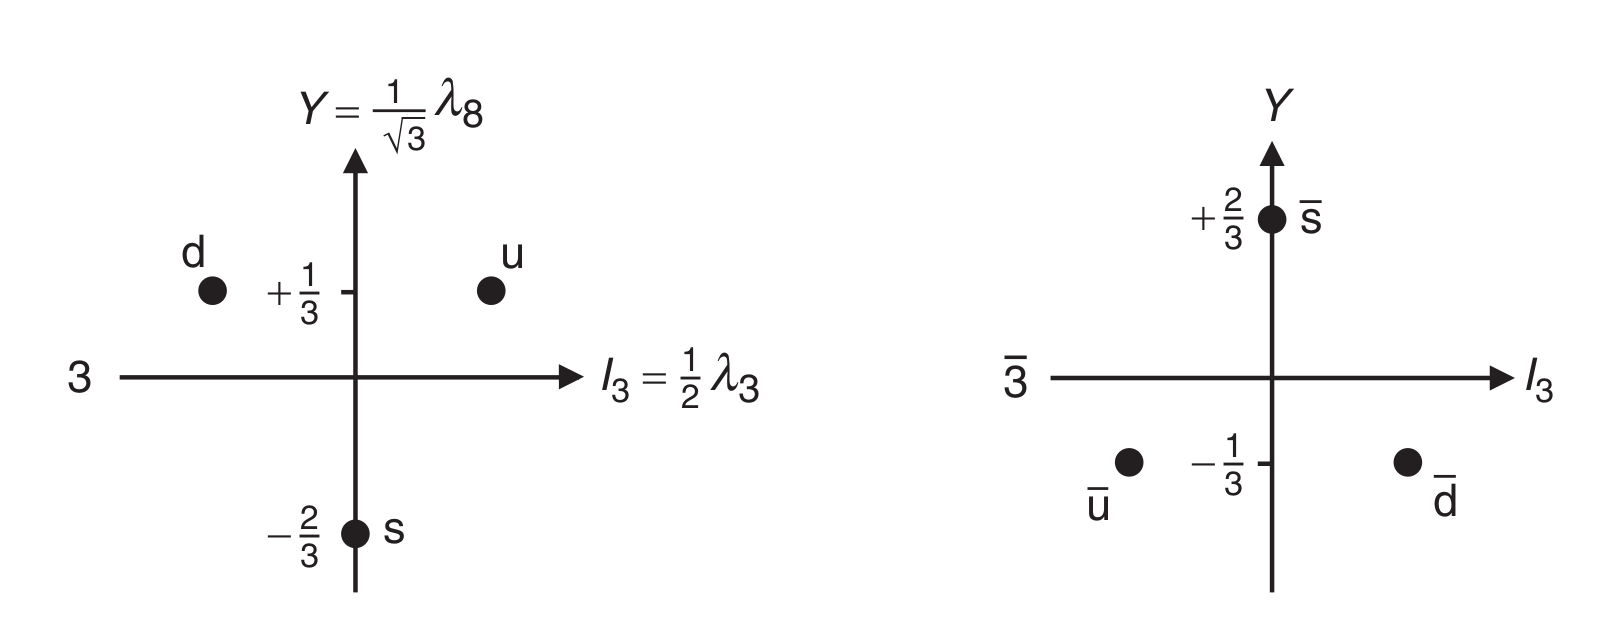
\includegraphics[width=0.6\textwidth]{Hypercharge.png}
\caption{\label{trailer}\emph{Quark Isospin and Hyper-charge}}
\end{figure}  
\end{itemize}
% subsection su3 (end)

\subsection{Light Mesons} % (fold)
\label{sub:light_mesons}
\begin{itemize}
\item Since we have used $\lambda_3$ and $\lambda_8$ to form what is know as the Cartan sub-algebra, we can take the remaining $\lambda_i$ and form raising and lowering operators. There will be three pairs, that which step respectively between the $d \leftrightarrow u, s\leftrightarrow u$ and $d\leftrightarrow s$:
\begin{align}
    \hat{T}_\pm &= \frac{1}{2} (\lambda_1 \pm i \lambda_2) \\
    \hat{V}_\pm &= \frac{1}{2} (\lambda_4 \pm i \lambda_5) \\
    \hat{U}_\pm &= \frac{1}{2} (\lambda_6 \pm i \lambda_7)
\end{align}
We can use these to find all possible Mesons made out of these $3$ quarks. This is done by identifying the extreme states (stats with maximal $I_3$ or $Y$), then apply the raising and lowering operators to exhaust all other possible states. Since we are combining $3$ possible quarks with $3$ possible anti-quarks \footnote{Here we are only looking at 2 quark combinations here, i.e. Mesons} then this is a case of $3 \otimes \bar{3} = 8 \oplus 1$ \footnote{The bar on the $3$ just indicates that this is the anti-quark triplet}. This decomposition is into a octet and a singlet and takes the below visual form:
 \begin{figure}[H]
\centering
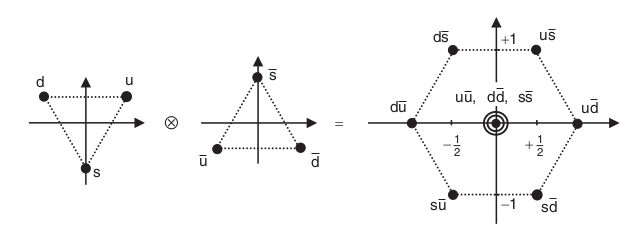
\includegraphics[width=0.5\textwidth]{3x3}
\caption{\label{trailer}\emph{Decomposition of quark-anti-quark combinations }}
\end{figure} 
Where the singlet is plotted along with the two octet elements that have $I_3 = Y = 0$. These quark combinations are as we mentioned before Mesons! We now have generated more of these having considered the strange quark as well. We are not how-ever considering spin. Quarks are spin $1/2$ particles meaning it is possible to form spin $0$ or spin $1$ combinations of them. It turns out that these different combinations affect the mass of the resulting bound system, meaning these are different particles. We thus have two sets of $9$ particles:
 \begin{figure}[H]
\centering
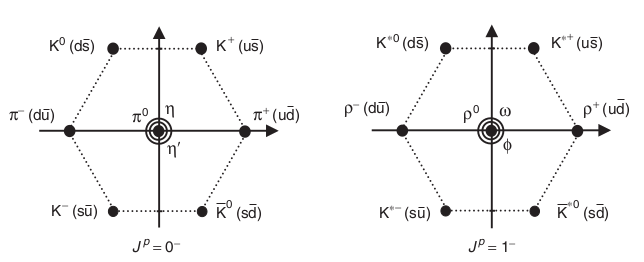
\includegraphics[width=0.6\textwidth]{mesons}
\caption{\label{trailer}\emph{All Mesons, graphed by Isospin and Hyper-charge}}
\end{figure} 
\item In terms of the quarks these are for spin-$0$:
\begin{align*}
    &\text{Pions:} 
    &|\pi^+\rangle = |u\bar{d}\rangle, \quad 
    |\pi^0\rangle = \frac{1}{\sqrt{2}} (|u\bar{u}\rangle - |d\bar{d}\rangle), \quad
    |\pi^-\rangle = |d\bar{u}\rangle \\[5pt]
    &\text{Kaons:} 
    &|K^+\rangle = |u\bar{s}\rangle, \quad
    |K^0\rangle = |d\bar{s}\rangle, \quad
    |\bar{K}^0\rangle = |s\bar{d}\rangle, \quad
    |K^-\rangle = |s\bar{u}\rangle \\[5pt]
    &\text{Eta and Eta Prime:} 
    &|\eta\rangle = \frac{1}{\sqrt{6}} (|u\bar{u}\rangle + |d\bar{d}\rangle - 2|s\bar{s}\rangle), \quad
    |\eta'\rangle = \frac{1}{\sqrt{3}} (|u\bar{u}\rangle + |d\bar{d}\rangle + |s\bar{s}\rangle)
\end{align*}
\item And for the spin-$1$ mesons:
\begin{align*}
    &\text{Rho Mesons:} 
    &|\rho^+\rangle = |u\bar{d}\rangle, \quad 
    |\rho^0\rangle = \frac{1}{\sqrt{2}} (|u\bar{u}\rangle - |d\bar{d}\rangle), \quad
    |\rho^-\rangle = |d\bar{u}\rangle \\[5pt]
    &\text{Kaon* Mesons:} 
    &|K^{*+}\rangle = |u\bar{s}\rangle, \quad
    |K^{*0}\rangle = |d\bar{s}\rangle, \quad
    |\bar{K}^{*0}\rangle = |s\bar{d}\rangle, \quad
    |K^{*-}\rangle = |s\bar{u}\rangle \\[5pt]
    &\text{Omega and Phi Mesons:} 
    &|\omega\rangle = \frac{1}{\sqrt{2}} (|u\bar{u}\rangle + |d\bar{d}\rangle), \quad
    |\phi\rangle = |s\bar{s}\rangle
\end{align*}
\item The Heavy Mesons are constructed from the bottom and charm quarks in a similar way. 
\end{itemize}
% subsection light_mesons (end)

\subsection{Baryons} % (fold)
\label{sub:baryons}
\begin{itemize}
    \item Baryons are combinations of $3$ quarks/ anti-quarks. This makes them fermions of spin $\frac{1}{2}$ or $3/2$. This means we need to calculate $3 \otimes 3 \otimes 3$. It turns out that the calculation of $3 \otimes 3$ is a little different to that of $3 \otimes \bar{3}$. Since we dont have anti-quarks we can't properly form a state that has $I_3=Y_3 =0$. This means the decomposition is $3 \otimes 3 = 6 \oplus 3$. This can be prooved by the standard ladder operator calculations. We are then left with $3 \otimes \left(6 \oplus 3\right)$ which breaks down into the standard $3 \otimes \bar{3} = 8 \oplus 1$ and the new $3 \otimes 6 = 10 \oplus 8$. Overall this means the full decomposition is:
\begin{flalign*}
    3 \otimes 3 \otimes 3 = 10 \oplus 8 \oplus 8 \oplus 1
\end{flalign*}
\item We can visulze this nicely with the followong:
    \begin{figure}[H]
\centering
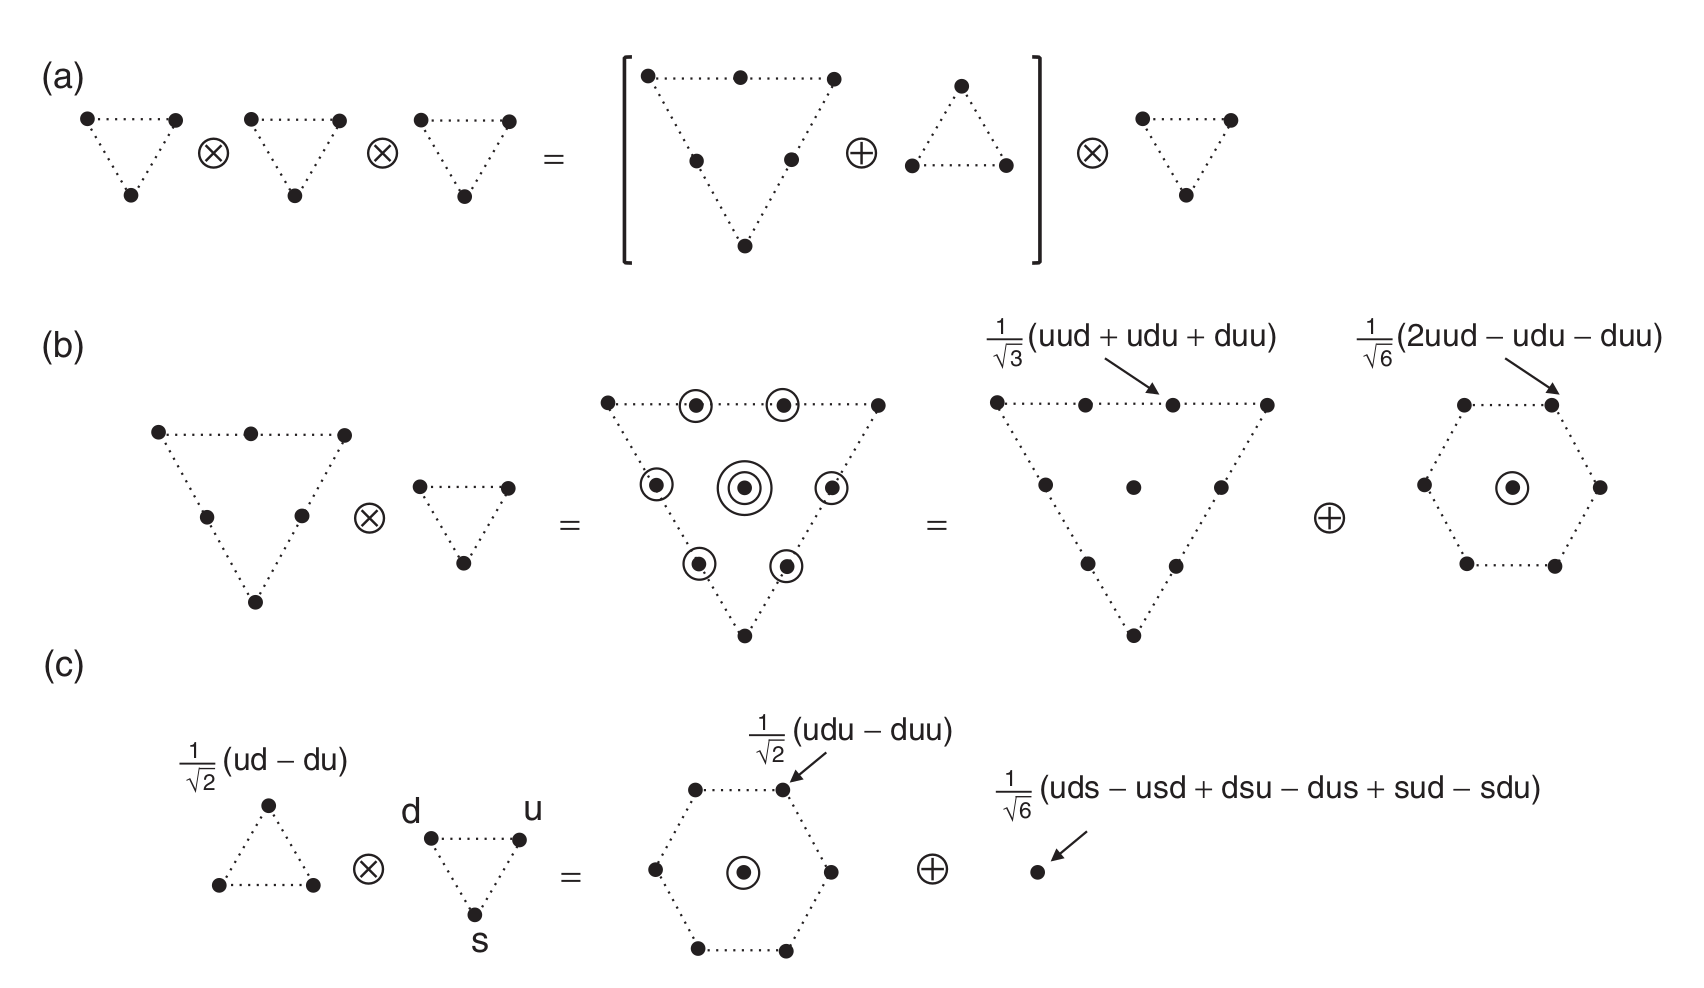
\includegraphics[width=0.8\textwidth]{3x3x3}
\caption{\label{trailer}\emph{All Mesons, graphed by Isospin and Hyper-charge}}
\end{figure}
\item The quark composition of the individual Baryons is then:
\begin{align*}
    &\text{Nucleons:} 
    &|p\rangle = |uud\rangle, \quad 
    |n\rangle = |udd\rangle \\[5pt]
    &\text{Delta Baryons:} 
    &|\Delta^{++}\rangle = |uuu\rangle, \quad
    |\Delta^+\rangle = |uud\rangle, \quad
    |\Delta^0\rangle = |udd\rangle, \quad
    |\Delta^-\rangle = |ddd\rangle \\[5pt]
    &\text{Sigma Baryons:} 
    &|\Sigma^+\rangle = |uus\rangle, \quad
    |\Sigma^0\rangle = |uds\rangle, \quad
    |\Sigma^-\rangle = |dds\rangle \\[5pt]
    &\text{Xi Baryons:} 
    &|\Xi^0\rangle = |uss\rangle, \quad
    |\Xi^-\rangle = |dss\rangle \\[5pt]
    &\text{Omega Baryon:} 
    &|\Omega^-\rangle = |sss\rangle
\end{align*}
\end{itemize}
% subsection baryons (end)
\subsection{Total Wavefunction} % (fold)
\label{sub:total_wavefunction}
\begin{itemize}
    \item There are many possible values of flavour, spin and colour (which we will encounter later) that a Baryon can have:
    \begin{align*}
        \psi = \phi_{\text{flavour}}\chi_{\text{spin}}\xi_{\text{colour}}\eta_{\text{space}}
    \end{align*}
    However, not all of these states are valid as since baryons are fermions, there total wave-functions needs to be anti-symmetric under exchange of any two quarks. We will see later that the colour wavefunction $\xi_{\text{colour}}$ is totally anti-symmetric. We are discussing the quarks with $l=0$, so zero spatial angular momentum , and since the spatial wavefunction transforms by $(-1)^l$ under parity, then $\eta_{\text{space}}$ is symmetric. This means that $ \phi_{\text{flavour}}\chi_{\text{spin}}$ must be symmetric. This allows us to determine the wave-function super positions of the quarks in terms of their flavour and spin. 
\end{itemize}
% subsection total_wavefunction (end)



\newpage
\section{Scattering \& Decay} % (fold)
\label{sec:scattering}
\begin{itemize}
    \item We will need to develop some mathematical tools for studying scattering of particles and Decay.
\end{itemize}

\subsection{Decay} % (fold)
 \label{sub:decay}
 \begin{itemize}
     \item Unstable particles have an equal probability of decaying at every instant in time. This means the probability of survival to time $t$ for a particle A is governed by:
     \begin{align*}
         &\frac{dP}{dt} = -\Gamma_A P \\
         \implies & P \propto e^{-\Gamma_At}
     \end{align*}
     The constant $\Gamma_A$ is known as the \emph{total width}. If there are multiple decay processes $A \rightarrow f$, then the total width is $\Gamma_A = \sum_f\Gamma(A \rightarrow f)$. The probability ratio of the decay into an individual particle $f$ is known as the \emph{branching ratio}: 
     \begin{align*}
         BR(A \rightarrow f) = \frac{\Gamma(A\rightarrow f)}{\Gamma_A} 
     \end{align*}
 \end{itemize}
 % subsection decay (end) 

 \subsection{Cross Section} % (fold)
 \label{sub:cross_section}
 \begin{itemize}
     \item The main object to interest to us in calculations will be the cross section, as this is measurable. Our scattering setup to calculate the cross section will be as follows. We consider a beam of A particles of density $n_A$ at a velocity $v_A$ at a target B:
\begin{figure}[H]
\centering
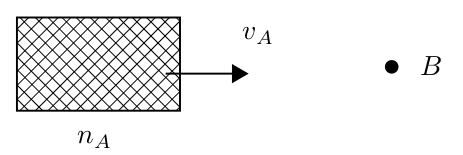
\includegraphics[width=0.6\textwidth]{scatter}
\caption{\label{trailer}\emph{Scattering setup}}
\end{figure}
\item The rate of scattering is then given by:
\begin{align*}
    \frac{\text{events}}{\text{sec}} = n_Av_A\sigma
\end{align*}
Where $\sigma$ is the cross section. It is useful for our calculations to consider all possible momenta the $n$ particles created in the process could have. The probability of finding each given momentum configuration of the final particles is given by the \emph{differential cross section}: $d\sigma/(d^3p_1 \cdot \cdot \cdot d^3p_n)$, which is related to the cross section by:
\begin{align*}
    \sigma = \int d^3p_1 \cdot \cdot \cdot d^3p_n\frac{d\sigma}{d^3p_1 \cdot \cdot \cdot d^3p_n}
\end{align*}

 \end{itemize}
 % subsection cross_section (end)

 \subsection{Master Formula} % (fold)
 \label{sub:master_formula}
 \begin{itemize}
     \item We know from our study of Quantum Field Theory \footnote{See my notes on QFT \href{https://tbrosnan12.github.io/documents/Fourth_year/First_semester/Quantum_Field_Theory_I.pdf}{here}.}, that the quantum mechanical transition matrix element is given by:
     \begin{align}
     \label{T_hat}
         \bra{12 \cdot \cdot \cdot n}T \ket{A(p_A)} = \mathcal{M}(A \rightarrow 1 +2 + \cdot \cdot \cdot n)(2\pi)^4\delta(p_A - \sum_jp_j)
     \end{align}
     Where $T$ is the time evolution operator. The factor of $\mathcal{M}$ is called the \emph{invariant Matrix element}. We will sometimes refer to it as the scattering amplitude. 
     \item To find the total rate of decay we need to integrate over the total phase, i.e. all momenta that the particles could have subject to the constraint of momentum conservation. This will be written as:
     \begin{align*}
          \int d\Pi_n = \int \frac{d^3p_1}{(2\pi)^32E_1} \cdot \cdot \cdot \frac{d^3p_n}{(2\pi)^32E_n}(2\pi)^4\delta(p_A - \sum_jp_j)
      \end{align*} 
Where we also for convenience have included in this the factors of $1/2E$, so as to satisfy Lorentz invariance.
\item Another formula we will then need from QFT is a version of Fermi's Golden rule, which tells us the particle width for a given transition to an $n-$particle final state $f$:
\begin{align*}
    \Gamma(A \rightarrow f) = \frac{1}{2m_A}\int d\Pi_n|\mathcal{M}(A\rightarrow f)|^2
\end{align*}
If the final products have spin we will need to sum over these spins. Similarly we need to do the same for the initial state, but often this state is unknown so we simply average over all possible spins instead. This expression is actually a simplification of the following more general expression for the cross section in therms of the invariant matrix element:
\begin{align}
\label{cross}
    \sigma(A+B \rightarrow f) = \frac{1}{2E_A2E_B|v_A-v_B|}\int d\Pi_n|\mathcal{M}(A\rightarrow f)|^2
\end{align}

 \end{itemize}
 % subsection master_formula (end)

 \subsection{2 Particle Collision} % (fold)
 \label{sub:2_particle_collision}
 \begin{itemize}
     \item We can now use the above equations to analyze the problem of a two particle collision. We will impotently do this for the case where $\mathcal{M}$ is constant, as this represents the case where each point in the phase space is equally likely. We will consider an initial state of momentum $P$ and a final state of two particles with momentum $\textbf{p}_1$ and $\textbf{p}_2$. In this scenario the phase space integral is just:
     \begin{align}
     \label{2_phase}
         \int \Pi_2 = \int \frac{d^3p_1}{(2\pi)^32E_1}\frac{d^3p_2}{(2\pi)^32E_2}(2\pi)^4\delta^{(4)}(P-p_1-p_2)
     \end{align}
 If we work in Center of Mass (CoM) frame, where $\textbf{P}=0$, then the three spatial parts of the delta function enforce that: $\textbf{p}_1=-\textbf{p}_2$ and thus if $P = (E_{\text{CM}},0) \implies p_1=(E_1,\textbf{p}) ~\&~ p_2=(E_2,-\textbf{p})$, where the particles are on shell so $E_1 = \sqrt{p^2+m_1^2}$ and $E_2 = \sqrt{p^2+m_2^2}$. With this \ref{2_phase} becomes:
     \begin{align}
     \label{2_phase_2}
         \int \Pi_2 = \int \frac{d^3p}{(2\pi)^3}\frac{2\pi}{2E_12E_2}\delta(E_{\text{CM}}-E_1-E_2)
     \end{align}
     In spherical co-ords this volume element is just $d^3p=p^2dpd\Omega$. We can then deal with this integral by using the property of the delta function for a function with only one zero at $x_0$:
     \begin{align*}
         &\delta(f(x)) = \frac{1}{|f'(x_0)|}\delta(x-x_0) \\
         \implies  & \delta(E_{\text{CM}}-E_1(p)-E_2(p)) = \frac{\delta(p-\tilde{p})}{|dE_1/dp+dE_2/dp|}
     \end{align*}
         We can evaluate from the on-shell conditions that $dE_1/dp = p/E_1$ and $dE_2/dp = p/E_2$, so we can write \ref{2_phase_2} as:
     \begin{align*}
          \int \Pi_2 &= \int \frac{\tilde{p}^2d\Omega}{16\pi^2E_1E_2}\frac{1}{|\tilde{p}/E_1+\tilde{p}/E_2|} = \frac{1}{E_1+E_2}\int \frac{\tilde{p}d\Omega }{16\pi^2} 
     \end{align*}
     \begin{flalign}
     \label{phase_2}
         = \frac{1}{8\pi}\left(\frac{2\tilde{p}}{E_{\text{CM}}}\right)\int\frac{d\Omega}{4\pi} 
     \end{flalign}
     We can note that in the relativistic limit $E>>m_1,m_2 \implies E_{\text{CM}} = E_1+E_2 \approx \tilde{p}+\tilde{p} =2\tilde{p}$, which makes the factor in brackets in \ref{phase_2} unity. This means \ref{phase_2} becomes constant in the relativistic limit. 
 \end{itemize}
 % subsection 2_particle_collision (end)
% section scattering (end)

\newpage
\section{Electron Positron Annihilation} % (fold)
\label{sec:electron_positron_annihilation}
\begin{itemize}
    \item We would now like to discuss the annihilation of an electron $e^-$ and its anti-particle the positron $e^+$. Firstly we will calculate the cross section for the process $e^+e^- \rightarrow \mu^+\mu^-$ ($\mu$ being muons) as this calculation will serve as a basis for many more complicated calculations. In doing this we will once again rely heavily on my QFT notes as we need to work with spinors for the fermions. 
\end{itemize}

\subsection{Feynman Diagrams} % (fold)
\label{sub:feynman_diagrams}
\begin{itemize}
    \item Despite their pretty form, Feynman diagrams do not represent physical process that actually happen. Despite this we will still use them for the basis of figuring out which terms in the expansion of the interaction part of the scattering which (as per section $8.4$ of my QFT notes) takes the form:
    \begin{align}
    \label{scattering_series}
        {}_{\text{in}}\braket{\textbf{p}_1\textbf{p}_2|\textbf{k}_{\mathcal{A}}\textbf{k}_{\mathcal{B}}}_{\text{out}} \propto \lim_{t\rightarrow\infty(1-i\epsilon)}{}_{0}\bra{\textbf{p}_1\textbf{p}_2}T\left\{\text{exp}\left(-i\int_{-t}^{t}dt'H_{I}(t')\right)\right\}\ket{\textbf{k}_{\mathcal{A}}\textbf{k}_{\mathcal{B}}}_{0}
    \end{align}
    We will expand in powers of the interaction parameter. The Lagrangian for QED (also per my QFT notes, see section 9.1) is given by\footnote{Note here the Dirac adjoint which is the bar on some of the $\psi$'s is defined as $\bar{\psi} \equiv \psi^{\dagger}\gamma^{0}$.}:
    \begin{align}
    \label{L_QED}
          \mathcal{L}_{\text{QED}} = -\frac{1}{4}F_{\mu\nu}F^{\mu\nu} +\bar{\psi}(i\gamma^{\mu}\partial_{\mu}-m)\psi - e\bar{\psi}\gamma^{\mu}\psi A_{\mu}
     \end{align}
     
     \item We will be working, for simplicity, in the high energy regime, where all particles in the $e^+e^- \rightarrow \mu^+\mu^-$ reaction can be treated as massless. Recall that the $\psi$'s here are Dirac fermions, which are comprised of two $2$-component spinors know as Weyl spinors. This spinors are called left and right handed spinors and the $\psi$'s which are $4$-component spinors can be written as the following \footnote{For a full discussion of Weyl spinors see section $4.6$ of my QFT notes.}:
     \begin{align*}
        \psi = \begin{pmatrix}
        \psi_L \\
        \psi_R
    \end{pmatrix}
\end{align*}
Note that for this calculation it is most useful to use the Chiral representation of the Dirac gamma matrices. This means\footnote{Note here $\bar{\sigma} = (\mathbbm{1},-\boldsymbol{\sigma})$}:
\begin{align*}
\gamma^{\mu} = \begin{pmatrix}
        0 & \sigma^{\mu} \\
        \bar{\sigma}^{\mu} & 0
      \end{pmatrix} \implies 
    \gamma^{0} = \begin{pmatrix}
      0 & \mathbb{I} \\
      \mathbb{I} & 0 
    \end{pmatrix},  ~~~ \gamma^{i} = \begin{pmatrix}
      0 & \sigma^{i} \\
      -\sigma^{i} & 0 
    \end{pmatrix} 
\end{align*}
\item With this we can see that the QED Lagrangian \ref{L_QED} can be expanded in terms of the left and right component spinors: 
\begin{align*}
    \mathcal{L}_{\text{QED}} = -\frac{1}{4}F_{\mu\nu}F^{\mu\nu} +i\psi_{R}^{\dagger}\sigma^{\mu}\partial_{\mu}\psi_R+i\psi_{L}^{\dagger}\bar{\sigma}^{\mu}\partial_{\mu}\psi_L - e\psi^{\dagger}_R\sigma^{\mu}\psi_RA_{\mu}- e\psi^{\dagger}_L\bar{\sigma}^{\mu}\psi_LA_{\mu}& \\
    + m\left(\psi^{\dagger}_R\psi_L + \psi^{\dagger}_L\psi_R\right)&
\end{align*}
From this we can see that the last term, which is proportional to the mass, couples the left handed spinors to the right handed ones. In fact if we have $m=0$, which is indeed the situation we will be considering, then the two left and right handed particles completely decouple and act as separate particles. This means in the high energy case a right handed electron cannot turn into a left handed one. Note that both species of particles also have their own interaction terms so they still interact amongst themselves. This isolation is essentially \emph{Conservation of helicity}. 

\item We are now ready to consider the interactions. Recall that in the calculation of terms in the power series of \ref{scattering_series} we contract ingoing and outgoing states with intermediate states. Since the interaction terms contain 3 fields, in order to have an even number of fields to contract we need to look at the quadratic terms of the interaction Hamiltonian $H_{I}$. This allows us to immediately write down the Feynman diagram that correspond to the first order interaction terms. We can reason that the following diagram is the only first order term as the fields available for contraction are $\bar{\psi},A,\psi,\bar{\psi},A,\psi$. Two of the $\psi$'s contract with the ingoing momenta and two with the outgoing in order to achieve $e^+e^- \rightarrow \mu^+\mu^-$, the final $A$'s must contract with themselves. This takes the following diagrammatic form: 
\begin{figure}[H]
\centering
    \resizebox{0.2\textwidth}{!}{
\begin{feynman}
    \fermion[label=\raisebox{-20mm}{\hspace{-5mm}$e^-$}]{4.00, 4.00}{5.00, 5.00}
    \fermion[label=\raisebox{-20mm}{\hspace{-4mm}$e^+$}]{6.00, 4.00}{5.00, 5.00}
    \electroweak[]{5.00, 5.00}{5.00, 6.00}
    \fermion[label=\raisebox{-20mm}{\hspace{-55mm}$\mu^-$},flip=true]{6.00, 7.00}{5.00, 6.00}
    \fermion[label=\raisebox{-20mm}{\hspace{21mm}$\mu^+$},flip=true]{4.00, 7.00}{5.00, 6.00}
\end{feynman}
    }
\end{figure}
\end{itemize}
\subsubsection{Massless Fermions} % (fold)
\label{ssub:massless_fermions}
\begin{itemize}
    \item In the case of $m=0$ fermions The Dirac equation $(i\gamma^{\mu}\partial_{\mu}-m)\psi = 0$ reduces to the following equations on the two spinors:
    \begin{align*}
         i\sigma^{\mu}\partial_{\mu}&\psi_{L} = 0 \\
      i\bar{\sigma}^{\mu}\partial_{\mu}& \psi_{R} =0 
    \end{align*}
    This means the solutions will take the following form (there are two types of solutions):
    \begin{align}
    \label{spinor_ansatz}
        &\psi_{R} = u_{R}(p)e^{-ip \cdot x}, ~~~ \psi_{L} = u_{L}(p)e^{-ip \cdot x}
    \end{align}
    Here the $u_R(p)$ and $u_L(p)$  are two component spinors that must satisfy their own versions of the Dirac equation. If we consider only plane waves propagating in the $\hat{z}$ direction, so $p = (E,0,0,p_z)$ then this equation is:
    \begin{align*}
         & (E-p_z\sigma_3)u_R = \begin{pmatrix}
             E-p_z & 0  \\
             0 & E+ p_z
         \end{pmatrix}u_R = 0  \\
         & (E+p_z\sigma_3)u_L = \begin{pmatrix}
             E+p_z & 0  \\
             0 & E- p_z
         \end{pmatrix}u_L = 0  
     \end{align*} 
     Both of these have the same solutions $\begin{pmatrix}
         1 \\ 0
     \end{pmatrix}$ and $\begin{pmatrix}
         0 \\ 1
     \end{pmatrix}$. When $u_R = \begin{pmatrix}
         1 \\ 0
     \end{pmatrix}$ it has $E = p_z >0$ and when $ = \begin{pmatrix}
         0 \\ 1
     \end{pmatrix}$ it has $E = p_z<0$. In the case of $u_L$ it is the other way round. It is convenient (see section 4.8 of my QFT notes) to normalize these spinors by $\sqrt{2E}$ and write them in the following:
     \begin{align*}
          & u_R = \sqrt{2E}\xi_+, ~~~u_L = \sqrt{2E}\xi_- \\
          & v_R = \sqrt{2E}\xi_-, ~~~v_L = \sqrt{2E}\xi_+
      \end{align*}    
      Where we have change $u \rightarrow v$ for the negative energy solutions. 

\item Big disclaimer, $\xi_+$ and $\xi_-$ are defined to be one of the two solution $(1,0)^T$ and $(0,1)^T$, how-ever the choice of which one they are depends on the direction of motion. $\xi_+$ is defined to be the spinor with spin up (that means positive eigenvalue) along the direction of motion and $\xi_-$ as the spinor with spin down (negative eigenvalue). However, we need to be careful in annihilation processes as then anti-particles are travailing the opposite direction and thus which spinor $(1,0)^T$ or $(0,1)^T$ has positive eigenvalue can swap. 

\item We can also do this for the more general case where the momentum is not along one of the axis. This will be relevant as we would like to be able to calculate the differential cross section as a function of angular variables. The picture of this in application to $e^+e^- \rightarrow \mu^+\mu^-$ is shown below:
\begin{figure}[H]
\centering
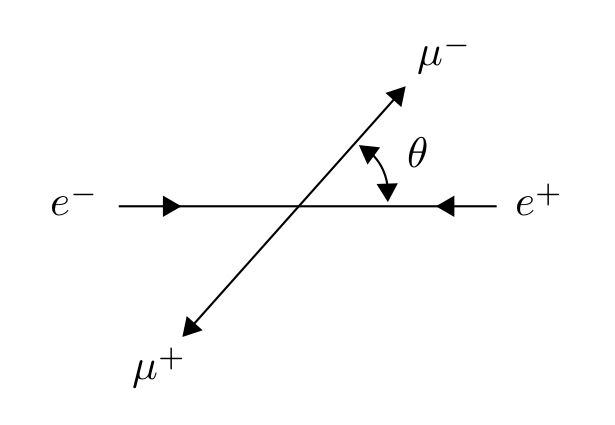
\includegraphics[width=0.5\textwidth]{e_mu}
\caption{\label{scatter}\emph{$e^+e^- \rightarrow \mu^+\mu^-$ process at angle $\theta$}}
\end{figure}
With the above setup we can see that the (massless) muons have the following momentum vectors (when the electron and positron are along the z axis):
\begin{align*}
    &p_-' = (E,E\sin\theta,0,E\cos \theta)\\
    &p_+' = (E,-E\sin\theta,0,-E\cos \theta)
\end{align*}
With this the spinor ansatz \ref{spinor_ansatz} equation for $u_R$ and $u_L$ become one of:
\begin{align*}
    &(E \pm E\sin \theta \sigma_x \pm E \cos \theta \sigma_z)u(p) = 0 \\
     &\implies \begin{pmatrix}
          1\pm \cos \theta & \pm \sin \theta \\
          \pm \sin \theta & 1\mp \cos \theta 
     \end{pmatrix}u(p) = 0 
\end{align*}
We can then solve for $u(p)$ in the following way. If $u(p) = (a ,b)^{T}$ then the top row reads:
\begin{align*}
    &(1 \pm \cos \theta)a \pm \sin \theta b =0 \hspace{-15mm}&\implies  a = \frac{\mp \sin \theta}{1 \pm \cos \theta}b \\
    & \text{plus case:}  & \text{minus case:} \\
    & a= \frac{2\cos \frac{\theta}{2}\sin \frac{\theta}{2}}{1+(\sin^2 \frac{\theta}{2} - \cos^2\frac{\theta}{2})} b& \hspace{-40mm}   a=  \frac{-2\cos \frac{\theta}{2}\sin \frac{\theta}{2}}{1-(\sin^2 \frac{\theta}{2} - \cos^2\frac{\theta}{2})}b \\
    & = \frac{2\cos \frac{\theta}{2}\sin \frac{\theta}{2}}{2\cos^2\frac{\theta}{2}}b & = \frac{-2\cos \frac{\theta}{2}\sin \frac{\theta}{2}}{2\sin^2\frac{\theta}{2}}b \\
    & = \frac{\sin \frac{\theta}{2}}{\cos \frac{\theta}{2}}b & = \frac{\cos \frac{\theta}{2}}{\sin \frac{\theta}{2}}b
\end{align*}
With this we can see that going to functions of $\theta/2$ has allowed us to find clearly normalized solutions for $u(p)$. These spinors are the new $\xi_+$ and $\xi_-$:
\begin{align}
\label{angular_spinors}
     \begin{pmatrix}
         \sin \frac{\theta}{2} \\ \cos \frac{\theta}{2}
     \end{pmatrix}, ~~~~~\begin{pmatrix}
         \cos \frac{\theta}{2} \\ -\sin\frac{\theta}{2}
     \end{pmatrix}
 \end{align} 
\end{itemize}
% subsubsection massless_fermions (end)
% subsection feynman_diagrams (end)


\subsection{Matrix Element} % (fold)
\label{sub:matrix_element}
\begin{itemize}
    \item The setup for the scattering in the Center of Mass (CM) frame will be the following. The electron and the positron will be moving in the opposite directions along the $\hat{z}$ axis with momenta $p_-$ and $p_+$. This means $p_- = (E,0,0,E)$ and $p_+ = (E,0,0,-E)$. The outgoing muon and anti-muon can be scattered at angles in the $\hat{x}-\hat{z}$ plane. Hence their outgoing momenta are given by $p_-' = (E,E\sin \theta,0,E\cos \theta)$ and $p_+' = (E,-E\sin \theta,0,-E\cos \theta)$.

    \item We can then use Feynman rules for QED (see section 9.2 of my QFT notes). Let us first deal with the annihilation of the electron and positron vertex. The Feynman rules tell us to add to our Matrix element a $-e\gamma^{\mu}$ for every vertex, note that in our case since we have split our Lagrangian into right and left handed spinors we instead add a $-e\sigma^{\mu}$ for right handed spinors and $-ie\bar{\sigma}^{\mu}$ for left handed spinors. We then have the contraction of the fields with the incoming momenta. One of the fields is a $\psi^{\dagger}$ \footnote{Note this is not a $\bar{\psi}$ here as we used the $\gamma^{0}$ from the $\bar{\psi}$ to make $\gamma^{\mu}$ diagonal so that the vertex cleanly gave us $\sigma^{\mu}$ and $\bar{\sigma}^{\mu}$.} this contracts with the incoming momenta of the positron to give us a $v^{\dagger}(p_+)$ as per the Feynman rules. Similarly the $\psi$ contracts with the incoming momenta of the electron to give us a $u(p_-)$. Mathematically this looks like the following. We will pick to do this for the case of a right handed electron and left handed positron\footnote{Note jsut as we mentioned earlier since the positron is going in the opposite direction $v_L^{\dagger}(p_+) = (0~1)^{T}$}.:
    \begin{align*}
        \bra{0}- e\psi^{\dagger}_R\sigma^{\mu}\psi_R\ket{e_R^{-}(p_-)e_L^{+}(p_+)} &=  \bra{0}\wick{- e\c1 \psi^{\dagger}_R\sigma^{\mu}\c2 \psi_R\ket{\c2e_R^{-}(p_-) \c1e_L^{+}(p_+)}} = -ev_L^{\dagger}(p_+)e^{-ip_+\cdot x}\sigma^{\mu}u_R(p_-)e^{-ip_-\cdot x} \\
         & = -e\sqrt{2E}(0 , 1)(1,\boldsymbol{\sigma})\sqrt{2E}\begin{pmatrix}
             1 \\0 
         \end{pmatrix}e^{-i(p_-+p_+)\cdot x} = -e2E(0,1,i,0)^{\mu}e^{-i(p_-+p_+)\cdot x}
    \end{align*}
    This vector we see here is nothing more then a polarization vector that we use to describe photons. We will call it $\epsilon^{\mu}_1 = (0,1,i,0)^{\mu}$. Note that the left handed current $- e\psi^{\dagger}_L\sigma^{\mu}\psi_L$ when acted on this electron positron ket is zero as in the massless case the right handed electron does not couple to the left handed fermions. 

    \item Next up is the propagator, which corresponds to the contraction of the two $A_{\mu}$ fields. This propagator in momentum space is given simply by \footnote{Note their is implicit time ordering operators on all quantities in this section. } (see section 4.8 of my QFT notes):
    \begin{align*}
       \bra{0} A_{\mu}(x) A_{\nu}(y)\ket{0}=\wick{\c A_{\nu}\c A_{\mu}} = \frac{-i\eta_{\mu\nu}}{q^2}e^{-iq \cdot (x - y)}
     \end{align*}
     \item Finally we have the contraction of the fields with the final muon momenta. This takes the following form, where we have used the angular versions of $\xi_+.\xi_-$ as sen in \ref{angular_spinors}:  
     \begin{align*}
         &\bra{\mu_R^{-}(p_-')\mu_L^{+}(p_+')}(- e)\psi^{\dagger}_R\sigma^{\nu}\psi_R \ket{0}=-e \wick{  \langle \c1\mu_R^{-}(p_-')\c2 \mu_L^{+}(p_+')| \c2 \psi^{\dagger}_R\sigma^{\nu}\c1 \psi_R}\ket{0} = -eu^{\dagger}_R(p_+')e^{ip_{+}'\cdot y}\sigma^{\nu}v_R(p_-')e^{ip_-'\cdot y} \\
         & = -e \sqrt{2E}(\sin \frac{\theta}{2} , \cos \frac{\theta}{2}) (1,\boldsymbol{\sigma})\sqrt{2E}\begin{pmatrix}
             \cos \frac{\theta}{2} \\ -\sin \frac{\theta}{2}
         \end{pmatrix} e^{i(p_+'+p_-')\cdot y} = -e2E( 0, \cos \theta, i, \sin \theta)^{\nu}e^{i(p_+'+p_-')\cdot y}
     \end{align*}
     Here we arrive at a different polarization vector $\epsilon_2^{\nu} = ( 0, \cos \theta, i, \sin \theta)^{\nu}$. 

     \item With all the pieces assembled we can now put them all together to calculate the contribution from the diagram:
     \begin{align*}
           \bra{\mu_R^{-}(p_-')\mu_L^{+}(p_+')}&(- e)\psi^{\dagger}_R\sigma^{\nu}\psi_R \ket{0}\bra{0} A_{\nu} A_{\mu}\ket{0}\bra{0}- e\psi^{\dagger}_R\sigma^{\mu}\psi_R\ket{e_R^{-}(p_-)e_L^{+}(p_+)} \\
           & = -e^2(2E)^2\epsilon_2^{\nu}\frac{i\eta_{\mu\nu}}{q^2}\epsilon^{\mu}_1e^{-i(p_-+p_+)\cdot x}e^{-iq \cdot (x - y)}e^{i(p_+'+p_-')\cdot y} \\
            & = -e^2(2E)^2\epsilon_2^{\nu}\frac{i\eta_{\mu\nu}}{q^2}\epsilon^{\mu}_1e^{-i(p_-+p_++q)\cdot x}e^{i(p_+'+p_-'+q)\cdot y}
     \end{align*}
     We can then remember that we are expanding in powers of the interacting Hamiltonian $H_I$ which is an integral over all space. This means we must integrate the above expression over all $x$ and $y$. We can see that the only $x$ and $y$ dependent terms are the exponentials, so these integral give us factors of $(2\pi)^4\delta^{(4)}(p_--p_+ -q)$ and $(2\pi)^4\delta^{(4)}(p_+'-p_-' +q)$. So we have:
     \begin{align}
     \label{2_delta}
         -2e^2(2E)^2\epsilon^{\ast\nu}_+\frac{i\eta_{\mu\nu}}{q^2}\epsilon^{\mu}_+(2\pi)^4\delta^{(4)}(p_-+p_+ +q)(2\pi)^4\delta^{(4)}(p_+'-p_-'+q)
     \end{align}

     Then we are required to integrate over all undetermined momenta, which is just integrating over $q$, this takes the two delta functions and requires that $p_-+p_+ = p_+'+p_-'$. which is just momentum conservation for the whole interaction. This also forces $q^2 = (p_-+p_+)^2 = (2E,0,0,0)^2 = (2E)^2$. All in all integrating \ref{2_delta} results in:
     \begin{align*}
          -e^2(\epsilon_2^{\nu}\eta_{\nu\mu}\epsilon_{1}^{\mu})(2\pi)^4\delta^{(4)}(p_-+p_+-p_+'-p_-')
     \end{align*}
      If we look at expression \ref{T_hat}, then we can see that this is exactly what we would expect to see from an interacting diagram, and that what is left over after the integration must be the matrix element $M$ for this $e^+e^- \rightarrow \mu^+\mu^-$ process. 

     \item Finally from their definitions we can see that $\epsilon_2^{\nu}\eta_{\nu\mu}\epsilon_{1}^{\mu} = 1+\cos\theta$. This means our matrix element for this particular $e^+e^- \rightarrow \mu^+\mu^-$ process is:
     \begin{align*}
         \mathcal{M}\left(e_L^+e_R^- \rightarrow \mu_L^+\mu_R^-\right) = -e^2(1+\cos \theta)
     \end{align*}
     Similarly one can do the same exact calculation we did here to get the other three amplitudes:
     \begin{align*}
         &\mathcal{M}\left(e_R^+e_L^- \rightarrow \mu_R^+\mu_L^-\right) = -e^2(1+\cos \theta) \\
        &\mathcal{M}\left(e_L^+e_R^- \rightarrow \mu_R^+\mu_L^-\right) = -e^2(1-\cos \theta) \\
        &\mathcal{M}\left(e_R^+e_L^- \rightarrow \mu_L^+\mu_R^-\right) = -e^2(1-\cos \theta)
     \end{align*}
\end{itemize}
% subsection matrix_element (end)

\subsection{Cross sections} % (fold)
\label{sub:cross_sections}
\begin{itemize}
    \item We can then directly use \ref{cross} to calculate the cross sections for each of these processes. For the phase space part of this integral we can use our previously calculated expression \ref{phase_2} for two particle collisions. In plugging into \ref{cross}, there is a little difficulty in figuring out what the velocities $|v_+-v_-|$ will look like if the particles are massless. for this we can simply recall that massless particles must move at the speed of light, which is $c=1$ in our units. So seeing as the initial electron and positron are moving in opposite directions, we have that $|v_+-v_-| =2$. This means the cross section for the $e_L^+e_R^- \rightarrow \mu_L^+\mu_R^-$ process is:
    \begin{align*}
        \sigma(e_L^+e_R^- \rightarrow \mu_L^+\mu_R^-) &= \frac{1}{2E2E \cdot 2}\int d\Pi_n|\mathcal{M}(e_L^+e_R^- \rightarrow \mu_L^+\mu_R^-)|^2 \\
        & = \frac{1}{16\pi E_{\text{CM}}^2}\int \frac{d \Omega}{4\pi} e^4(1+\cos \theta)^2
    \end{align*}
    This expression allows us to write down the differential cross section in terms of $\alpha \equiv \frac{e^2}{4\pi}$:
    \begin{align*}
         \frac{d \sigma}{d\Omega} =\frac{\alpha^2}{4E_{CM}^2}(1+\cos \theta)^2
     \end{align*}
     We find that if we average over the 4 possible processes then the differential cross section becomes:
     \begin{align*}
          \frac{d \sigma}{d\Omega} =\frac{\alpha^2}{4E_{CM}^2}(1+\cos^2 \theta)
      \end{align*} 
      Integrating this gives us the total cross section:
      \begin{flalign}
          \sigma(e^+e^- \rightarrow \mu^+\mu^-) = \frac{4\pi\alpha^2}{3E_{CM}^2}
      \end{flalign}
\end{itemize}
% subsection cross_sections (end)

\subsection{$e^+ e^- \rightarrow $ Hadrons} % (fold)
\label{sub:_e_e_rightarrow_hadrons}
\begin{itemize}
    \item The cross section we have just calculated can be very easily generalized to many other first order calculations where we also assume the that the particles involved are massless in the high energy limit. Take for example an electron and positron colliding to form hadrons. the only changes we need to make are $1:$ the value of the coupling $e \rightarrow Q_f e$ where $Q_f$ is the charge of the quark species in question \footnote{This only happens for two of the $4~e$'s in the final answer above above as there are 2 quarks, an electron and a positron, hence we get a factor of $Q_f^2$.}. $2$: to get the final cross section the set of all processes includes all possible quarks that we are considering so we must sum over them. The final result is simply:
    \begin{align*}
         \sigma(e^+e^- \rightarrow \text{hadrons}) =  \sum_f3Q_f^2\frac{4\pi\alpha^2}{3E_{CM}^2}
      \end{align*}  
      Note there is a mysterious factor of $3$ that has popped up here. This is due to the fact that quarks have another quantum number called colour which we will see later. There are $3$ colours and we must sum over them hence the factor of $3$. 
\end{itemize} 
% subsection _e_e_rightarrow_hadrons (end)
% section electron_positron_annihilation (end)


\newpage

\section{Deep Inelastic Scattering} % (fold)
\label{sec:deep_inelastic_scattering}
\begin{itemize}
    \item We will now be discussing processes that probes the structure of the proton (quarks gluons ect). This is done by electron positron scattering into electron plus some hadrons . The ``inelastic" refers to the fact that this process breaks the proton and produces hadrons, thus a high momentum transfer is needed. This high energy transfer is so large that the mass of the hadrons produced are $>>m_p$. The ``Deep" refers to the fact that this scattering probes the inner structure of the proton. The first interacting Feynman diagram for this process looks like the following:

\begin{figure}[H]
\centering
\resizebox{0.5\textwidth}{!}{
    \begin{feynman}
    \fermion[label=\raisebox{-27mm}{\hspace{-30mm}$e^-$}]{18.00, 7.00}{17.00, 8.00}
    \fermion[label=\raisebox{-15mm}{\hspace{-3mm}$e^-$}]{17.00, 6.00}{18.00, 7.00}
    \fermion[label=\raisebox{-25mm}{\hspace{16mm}Hadrons}, showArrow=true, flip=true]{21.00, 8.00}{20.40, 7.40}
    \fermion[label=\raisebox{-15mm}{\hspace{-5mm}$p$}]{21.00, 6.00}{20.40, 6.60}
    \electroweak[]{18.00, 7.00}{19.5, 7.00}
    \parton{20.00,7.00}{0.50}
\end{feynman}
}
\end{figure}

\item If the incoming electron has momentum $k$ and the outgoing photon momentum $k'$, then we know from conservation of momentum at the vertices of Feynman diagrams that the momentum carried by the photon $q$ is given by $q = k-k'$. This means for this scattering process if we look at the leading order where $m_e \rightarrow 0$, then $q^2 = -2k \cdot k'$, as $k$ and $k'$ are both light-like in opposite directions meaning $k^2=k'^2=m_e^2=0$ and hence $k \cdot k' = E^2+\textbf{k}\cdot\textbf{k}' = E^2 >0$. This makes $q^2<0$ i.e. space-like. With $q$ being space-like there is always a frame where the energy transfer is $0$ and there is only momentum transfer. Thus we define $Q^2 \equiv -q^2$ to be the momentum transferred.
\end{itemize}

\subsection{The Parton Model} % (fold)
\label{sub:the_parton_model}
\begin{itemize}
    \item A simple model posited by Feynman was to model the proton as being made of a collection of smaller constituents called partons. We can assume the partons are spin half quarks carrying a flavour label $f$ (or $\bar{f}$ for anti quarks). We assume at high energies the particle have momenta in line with the proton such that the transverse components are of the same order of the momenta with in the bound state of the proton. With this we can model each parton as having a fraction $\xi$ of the protons total momenta $P$:
    \begin{align*}
        p^{\mu} = \xi P^{\mu}
    \end{align*}
    The parameter $\xi$ must be $0 < \xi < 1$. We then define the \emph{Parton distribution functions} (PDFs) $f_f(\xi)d\xi$ as the probability of finding a parton of type $f$ caring momentum fraction $ \in (\xi,\xi+d\xi)$. Clearly these PDFs must satisfy a sum rule for the total momentum to be $P$: 
    \begin{align*}
        \int_0^1d\xi \sum_f\left[f_f(\xi) + f_{\bar{f}}(\xi)\right] =1
    \end{align*}
    We can then consider that the electrons interacts with each of the quarks in the proton and that the resulting cross section for the production of a hadron state $X$ is given by the sum over all possible interactions at all possible momenta:
    \begin{align*}
        \sigma(e^-p \rightarrow e^-X) = \int_{0}^{1}d\xi\sum_f\left[f_f(\xi)+f_{\bar{f}}(\xi)\right]\sigma(e^-q(\xi p)\rightarrow e^-q)
    \end{align*}
    Note here we are ignoring the effects of the strong interaction. Also we have written the cross section for the quark and anti-quark as the same as we know from our discussions at the end of the last chapter that the cross sections of electrons and quarks are proportional to the charge squared and thus do not depend on the sign.  
\end{itemize}
% subsection the_parton_model (end)

\subsection{Crossing Symmetry} % (fold)
\label{sub:crossing_symmetry}
\begin{itemize}
    \item We now wish to obviously calculate these cross sections. Before we blindly go into the calculations as we did in the last chapter we can stop to think is there anything clever we can do to leverage the hard work we did in the last chapter. If we draw the diagram for each of the electron quark interactions the firs order diagram is:  
    \begin{figure}[H]
\centering
\resizebox{0.4\textwidth}{!}{
    \begin{feynman}
    \fermion[label=\raisebox{-27mm}{\hspace{-30mm}$e^-$}]{18.00, 7.00}{17.00, 8.00}
    \fermion[label=\raisebox{-15mm}{\hspace{-3mm}$e^-$}]{17.00, 6.00}{18.00, 7.00}
    \fermion[label=\raisebox{-25mm}{\hspace{16mm}$q$}, showArrow=true, flip=true]{20.50, 8.00}{19.5, 7.00}
    \fermion[label=\raisebox{-15mm}{\hspace{-5mm}$q$}]{20.50, 6.00}{19.5, 7.00}
    \electroweak[]{18.00, 7.00}{19.5, 7.00}
\end{feynman}
}
\end{figure}
We can notice that this is just the interaction we considered at the end of the last chapter with a few changes (see the Feynman diagram at the top of pg 13 with the muons replaced with quarks). The changes are: instead of having an incoming positron we have and outgoing positron, similarly instead of having an out going anti-quark we have an outgoing quark. This is essentially rotates the diagram sideways (and flips it). It turns out that this change results in the exact same Matrix elements (only when squared ans summed over spins). The reason this is true is a little technical and I will leave the proof to (hopefully) be in my QFT notes. This symmetry is known as \emph{crossing symmetry}. 

  \item To use crossing symmetry it is useful to establish the following conventions and notation for 2 particle $\rightarrow$ 2 particle interactions. We can consider the general case where we don't know what the intermediate interaction looks like:
\begin{figure}[H]
\centering
\resizebox{0.3\textwidth}{!}{
    \begin{feynman}
    \fermion[label=\raisebox{-27mm}{\hspace{-30mm}$p_3$},flip=true]{19.00, 8.00}{19.60, 7.40}
    \fermion[label=\raisebox{-15mm}{\hspace{-3mm}$p_1$},flip=true]{19.00, 6.00}{19.6, 6.60}
    \fermion[label=\raisebox{-25mm}{\hspace{16mm}$p_4$}, showArrow=true,flip=true]{21.00, 8.00}{20.40, 7.40}
    \fermion[label=\raisebox{-15mm}{\hspace{-5mm}$p_2$},flip=true]{21.00, 6.00}{20.40, 6.60}
    \parton{20.00,7.00}{0.50}
\end{feynman}
}
\caption{Crossing symmetry labeling}
\label{fig:cross}
\end{figure}
Note that for simplicity we have made all the momenta exiting the interaction so that conservation of momentum for the diagram reads $p_1+p_2+p_3+p_4=0$. When considering what makes up the invariant matrix element of a given must be made of Lorentz invariant quantities. Since the only inputs are the momenta, the only combinations we can have we denote with the following variables called the the \emph{Mandelstam variables}:
\begin{align*}
    s =(p_1+p_2)^2 = (p_3+p_4)^2 \\
    t = (p_1+p_3)^2 = (p_2+p_4)^2 \\
    u = (p_1+p_4)^2 = (p_2+p_3)^2 
\end{align*}
These are not all independent as it can be shown that $s+t+u = m_1^1+m_2^2+m_3^2+m_4^2$. 

\item To see how these variables can help us with crossing symmetry we can consider the scattering where particles $1$ and $2$ co-linearly scatter to form particles $3$ and $4$. 
\begin{figure}[H]
\centering
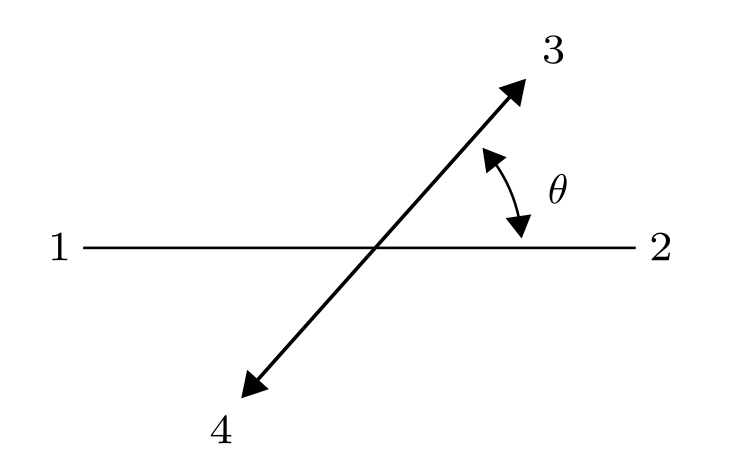
\includegraphics[width=0.5\textwidth]{1_2_scatter}
\end{figure}
With this we have that the momenta are:
\begin{align*}
    p_1 &= (-E,0,0,-E), ~~~&p_3 = (E,E\sin \theta,0,E\cos \theta) \\
    p_2 &= (-E,0,0,E), ~~~&p_4 = (E,-E\sin \theta,0,-E\cos \theta)   
\end{align*}
Note that since we have defined all the momenta to be exiting the diagram, particles $1$ and $2$ have negative energy. With this setup we have that:
\begin{align*}
    s &= (2E,0,0,0)^2  = E_{CM}^2 \\
    t &= (0,E\sin \theta,0,E(\cos\theta-1))^2 = -2E^2(1-\cos \theta) \\
    u &= (0,-E\sin\theta,0,-E(1+\cos\theta))^2 = -2E(1+\cos\theta)
\end{align*}
Also since we have used light-like momentum vectors $s+t+u=0$, which is expected as this should be equal to the sum of the masses which are in this case massless. 

\item With this setup we can use crossing symmetry to make our calculations a lot easier. Recall that the QED propagator contains a $1/(q^2-m^2)$, and thus final answer contained $1/(q^2-m^2)$, where $q^2$ by momentum conservation at the vertex must be $q^2 = (p_1+p_2)^2 \equiv s$ (as shown in the last section). This then means that annihilation diagrams correspond to:
\begin{align*}
        \begin{array}{c}
            \begin{tikzpicture}
    \begin{pgfonlayer}{nodelayer}
        \node [style=none] (0) at (0, 0) {};
        \node [style=none] (1) at (0, 1) {};
        \node [style=none] (2) at (-1, 2) {};
        \node [style=none] (3) at (1, 2) {};
        \node [style=none] (4) at (1, -1) {};
        \node [style=none] (5) at (-1, -1) {};
    \end{pgfonlayer}
    \begin{pgfonlayer}{edgelayer}
        \draw (5.center) to (0.center);
        \draw (4.center) to (0.center);
        \draw (0.center) to (1.center);
        \draw (1.center) to (2.center);
        \draw (1.center) to (3.center);
    \end{pgfonlayer}
\end{tikzpicture}
        \end{array} \sim \frac{1}{s-m^2}
    \end{align*}    
    This is subsequently known as an $s$ channel process. 

    \item We can then consider scattering, looking at the diagram below we can see that momentum conservation will make it so that $ q^2 = (p_1+p_3)^2 \equiv t$  (where we refer to the Figure \ref{fig:cross} for the labeling), thus we have:
    \begin{align*}
        \begin{array}{c}
            \begin{tikzpicture}
    \begin{pgfonlayer}{nodelayer}
        \node [style=none] (0) at (-1, 0) {};
        \node [style=none] (4) at (-2, 1) {};
        \node [style=none] (5) at (-2, -1) {};
        \node [style=none] (6) at (0, 0) {};
        \node [style=none] (7) at (1, 1) {};
        \node [style=none] (8) at (1, -1) {};
    \end{pgfonlayer}
    \begin{pgfonlayer}{edgelayer}
        \draw (4.center) to (0.center);
        \draw (5.center) to (0.center);
        \draw (0.center) to (6.center);
        \draw (6.center) to (7.center);
        \draw (6.center) to (8.center);
    \end{pgfonlayer}
\end{tikzpicture}
\end{array} \sim \frac{1}{t-m^2}
    \end{align*} 
    This is then known as a t channel process. 

    \item Finally there is one more, which is the same scattering but with the final states swapped, this then has $ q^2 = (p_1+p_4)^2 \equiv u$, so we get the $u$-channel process:
    \begin{align*}
        \begin{array}{c}
            \begin{tikzpicture}
    \begin{pgfonlayer}{nodelayer}
        \node [style=none] (0) at (-1, 0) {};
        \node [style=none] (5) at (-2, -1) {};
        \node [style=none] (6) at (0, 0) {};
        \node [style=none] (8) at (1, -1) {};
        \node [style=none] (13) at (-1, 1) {};
        \node [style=none] (14) at (0, 1) {};
        \node [style=none] (2) at (-.25, .25) {};
    \end{pgfonlayer}
    \begin{pgfonlayer}{edgelayer}
        % Lower part of crossing line
        \draw (5.center) to (0.center);
        \draw (0.center) to (6.center);
        \draw (6.center) to (8.center);
        % Upper part of main diagonal
        \draw (0.center) to (14.center);
        % Overlapping effect: use a white line to cover part of the main diagonal
        \draw[line width=2mm, white] (13.center) -- (2.center);
        % Foreground segment
        \draw (13.center) to (6.center);
    \end{pgfonlayer}
\end{tikzpicture}
\end{array} \sim \frac{1}{u-m^2}
    \end{align*} 
    \item With these identifications crossing symmetry becomes very easy! If we started with a $t$ channel process we can relate its amplitude to a $s$ channel annihilation by simply changing $s \leftrightarrow t$. 
\end{itemize}
% subsection crossing_symmetry (end)

\subsection{Electron Quark Scattering} % (fold)
\label{sub:electron_quark_scattering}
\begin{itemize}
    \item We are now prepared to write down our matrix elements for the deep inelastic scattering. We start by writing down the matrix elements of the electron positron annihilation into quarks. This we we discussed at the end of the last section, is just the same elements as the $e^-e^+ \rightarrow q_L\bar{q}_R$
    \begin{align*}
    &|\mathcal{M}\left(e_L^+e_R^- \rightarrow q_L^+\bar{q}_R^-\right)|^2 = |\mathcal{M}\left(e_R^+e_L^- \rightarrow q_R^+\bar{q}_L^-\right)|^2 = Q_f^2e^4(1+\cos \theta)^2 \\
        &|\mathcal{M}\left(e_L^+e_R^- \rightarrow q_R^+\bar{q}_L^-\right)|^2 =|\mathcal{M}\left(e_R^+e_L^- \rightarrow q_L^+\bar{q}_R^-\right)|^2= Q_f^2e^4(1-\cos \theta)^2 
     \end{align*}
     The next step is to write these in terms if the Mandelstam variables: 
          \begin{align*}
    &|\mathcal{M}\left(e_L^+e_R^- \rightarrow q_L\bar{q}_R\right)|^2 =|\mathcal{M}\left(e_R^+e_L^- \rightarrow q_R\bar{q}^-\right)|^2=  4Q_f^2e^4\frac{u^2}{s^2} \\
        &|\mathcal{M}\left(e_L^+e_R \rightarrow q_R\bar{q}_L\right)|^2 =|\mathcal{M}\left(e_R^+e_L^- \rightarrow q_L\bar{q}_R\right)|^2  = 4Q_f^2e^4\frac{t^2}{s^2} 
     \end{align*}
     This then immediately lets us write down the amplitudes for the $e^-q \rightarrow e^-q$ scattering. We have with this change of diagram that $p_1 \rightarrow p_1,~p_2\rightarrow p_3,~ p_3\rightarrow p_4, p_4 \rightarrow p_2$ as we simply just replace $s \rightarrow t,~t \rightarrow u,~u\rightarrow s$.  So we can write down the $4$ matrix elements:
     \begin{align*} 
    &|\mathcal{M}\left(e_R^-q_L \rightarrow e_R^-q_L\right)|^2 =|\mathcal{M}\left(e_L^-q_R \rightarrow e_L^-q_R\right)|^2=  4Q_f^2e^4\frac{s^2}{t^2} \\
        &|\mathcal{M}\left(e_L^-q_L \rightarrow e_L^-q_L\right)|^2 =|\mathcal{M}\left(e_R^-q_R \rightarrow e_R^-q_R\right)|^2  = 4Q_f^2e^4\frac{u^2}{t^2} 
     \end{align*}
     \item We can then calculate the cross sections as we did in the last section, using \ref{cross}, remembering that we are treating the particles as massless so $|v_A-v_B|=2$. We will then use relativistic limit of \ref{phase_2} to evaluate the phase space integral. This makes the cross section for each process take the form:
     \begin{align*}
         \sigma(\ldots)  &= \frac{1}{2E2E \cdot 2}\int d\Pi_n|\mathcal{M}(\ldots)|^2\\
          & =\frac{1}{16\pi E_{\text{CM}}^2}\int \frac{d \Omega}{4\pi}|\mathcal{M}(\ldots)|^2
     \end{align*}
     We then have to be careful about how we add up these amplitudes. There can only ever be two incoming spins, which we cannot know as the beams are not polarized, this means in order to match experiment we must average over initial spins. We do however want to know the cross section for all possible final spins, this means we must sum over the final spins. We do not sum over initial states as each spin configuration has equal probability of occurring, hence averaging is all that is needed. Similarly the outgoing spins already have the probabilities encoded with them via the matrix elements $\mathcal{M}$, so we do not need to average them further. 

      \item All this means for this calculation is that we sum over all the $\mathcal{M}$'s and divide by $4$ to average the initial states as they each only have one final state.  The total cross section is then:
      \begin{align*}
          \sigma(e^-q \rightarrow e^-q) &=  \frac{1}{16\pi E_{\text{CM}}^2}\int \frac{d \Omega}{4\pi}\frac{1}{4}\sum|\mathcal{M}(\ldots)|^2 \\
          & =  \frac{1}{16\pi E_{\text{CM}}^2}\int \frac{d \Omega}{4\pi}\frac{2}{4}\left(4Q_f^2e^4\frac{s^2+u^2}{t^2}\right) \\
          & = \frac{e^4}{16\pi}\frac{Q_f^2}{s}\int d \cos \theta \left(\frac{s^2+u^2}{t^2}\right)
      \end{align*}
      Where we have used the fact that $s=E_{\text{CM}}^2$. This means:
      \begin{align*}
           \frac{d\sigma}{d\cos\theta} = \frac{\pi\alpha^2}{s}Q_f^2\left(\frac{s^2+u^2}{t^2}\right)
      \end{align*}
      This can then nicely be written as the following using the fact that $ t= -2E^2(1-\cos \theta)  \implies dt = -\frac{1}{2}sd\cos\theta$:
      \begin{align*}
          \frac{d\sigma}{dt} = \frac{2\pi\alpha^2}{s^2}Q_f^2\left(\frac{s^2+u^2}{t^2}\right)
      \end{align*}
        

\end{itemize}
% subsection electron_quark_scattering (end)

% section deep_inelastic_scattering (end)
\end{document}
    